%%%%%%%%%%%%%%%%%%%%%%%%%%%%%%%%%%
%%%%%   ALTERNATIVE MODELS   %%%%%
%%%%%%%%%%%%%%%%%%%%%%%%%%%%%%%%%%
\chapter[Reverse catalytic models: analysis of seroprevalence]{Reverse catalytic models:\\ analysis of seroprevalence}
\label{ch:5.0}

% \textcolor{red}{Coisas a apontar pelo Nuno: devia ter lido mais para detectar gralhas/confusões em termso estatísticos. \textbf{JÁ:}peak-shift -- tenho de falar LOGO na introdução! Conceito não é geral (mais conhecido na parte da modelação matemática) Tem de estar claro na introdução.}
All analyses performed in this chapter used the seropositivity registered from the three specific \textit{P. falciparum} antimalarial antigens MSP1, MSP2, and AMA1, as the outcome of interest.
Focusing on these detected signals of exposure to malaria parasites brought new inference tools to the study of transmission intensity across the distinct sites.
% Shifting the analyses from recorded symptomatic cases, to these detected signals of exposure to malaria parasites through the antigens brings new inference tools -- seroepidemiological tools -- to the study of transmission intensity across different sites.
The nested reverse catalytic models (RCMs) were here applied to the data of each village.
% Each model estimates seroprevalence assuming individuals transit between seronegative and seropositive states for the different antigens.
The models' results were compared using the likelihood ratio tests, identifying the statistically overall best model for each village and antigen (parametric dependencies represented in Figure \ref{fig:lrt.rcm.models}).

Models considering a change in seroreversion rate (SRR), M$_{1,1}$ and the more restricted M$_{1,2}$, were proposed alongside this thesis.
Their results were compared beforehand, selecting the true model for the age-dependent change in SRR.
Afterwards, both models assuming changes in their transition rates were compared to M$_0$ with constant seroconversion rate (SCR) and SRR across all ages.
The application of different RCMs allowed for inferences on how the acquired immune system behaves upon exposure to a certain level of transmission intensity.
% Estimating malaria transmission rate through different RCMs allowed for inferences on how the immunological system behave when individuals are exposed to different levels of transmission to be made. \textcolor{red}{esta frase não está bem -- quero saber a intensidade de transmissão (frase anterior)}
Also, by tracking different antimalarial antibodies detected at different ages, the RCMs can explain the past serological history of the populations, describing if any noticeable change occurred in recent decades.
%can also bring epidemiological inferences can also be made.
%Analyses on how the gradual accumulation of different immunologic defences over years of exposure, or recent campaigns for malaria control can change transmission intensity.
%From the results one should be able to infer how the gradual accumulation of antigens over years of exposure can present an impact on transmission intensity.
%Also, how the campaigns for malaria control in recent decades helped shaping the immunological spectrum of the Northeast Tanzania populations, and what it means.
%the main focus from analysing the variables modelling the prevalence of infection to considering how such probability of disease can be modulated by serological recorded values, and how does it change throughout an individual's life.
%the effects of acquired immunity through continued exposure to the endemic disease.
%In this chapter, the previously described RCMs are put to use.
%Results for model M$_0$ are firstly described,
%Since all models are nested, the comparisons are made through the likelihood ratio test.

%%%%%%%%%%%
% RESULTS %
%%%%%%%%%%%
\section{Model results and comparison}
%%%%%%%%%%%%%
% M12 v M11 %
%%%%%%%%%%%%%
\subsection[Models for age-dependent seroreversion rate]{Models for age-dependent SRR: M$_{1,1}$ \textit{vs.} M$_{1,2}$}

Before comparing the different RCMs alongside their sero-epidemiological implications, both models assuming change in SRR were compared (Tables \ref{tab:M12.M11.msp1}, \ref{tab:M12.M11.msp2} and \ref{tab:M12.M11.ama1} from Appendices, for the antigens MSP1, MSP2, and AMA1, respectively).
Both models
%M$_{1,1}$ with restriction $\rho_2\leq\rho_1$, and M$_{1,2}$, with restriction $\rho_2=0$,
represented the individual biological effects of accumulated antimalarial immunity due to exposure, under stable and constant rate of transmission across all ages.
% Depending on the intensity, seronegative individuals transit into an antigen seropositive state.
% Considering an endemic scenario, exposed seropositive individuals remain in this state as long as the parasitic infections are recurrent.
The models assumed a reduction in SRR, $\rho_1$ to $\rho_2$, given an age cutoff $\uptau$.
% As more exposed individuals become seropositive, the models assume a reduction in seroreversion rate ($\rho_1$) to a obligatory lower rate ($\rho_2$), given the time cutoff.
However, while M$_{1,1}$ considered the reduction $\rho_1\geq\rho_2$, the more restricted M$_{1,2}$ assumed that after some age $\uptau$, all individuals had transited into the seropositive state ($\rho_2=0$), remaining so.
% , there remaining whilst the stable transmission endured.

% Results from the two models are compared (Tables \ref{tab:M12.M11.msp1}, \ref{tab:M12.M11.msp2}, and \ref{tab:M12.M11.ama1}, from Appendices, for antigens MSP1, MSP2, and AMA1, respectively).
When the models were fit to data from different antigens, $ \widehat{\rho}_2$ estimates from model M$_{1,1}$ were consistent with zero for some villages.
The likelihood ratio tests further validated the results, suggesting the model to be statistically equivalent to M$_{1,2}$ (p-value $>0.05$) for a majority of the villages.
When comparing both age-dependent SRR models, despite some villages being significantly better described by M$_{1,1}$, possible numeric errors registered in the estimates of this model (resulting in numerous estimates for $ \widehat{\rho}_1>10$) led to the choosing of M$_{1,2}$ as the best model to take further into the analyses.

With M$_{1,2}$ as the selected model, estimates for $ \widehat{\rho}_2$ equal to zero in every village suggested individuals persist as seropositive after some time, regardless of antigen or transmission intensity.
Within each transect, SCR estimates, $ \widehat{\lambda}$, seemed to decrease with altitude.
% From the SRR estimates, an altitude effect could also be inferred, although not as dependent as the previous parameter estimates.
Contrarily, the influence of altitude was positively related to $ \widehat{\rho}_1$, as lower estimates were generally found in villages located at low and intermediate altitudes.
Estimates for the cutoff parameter $ \widehat{\uptau}$ were consistently higher for lower altitude villages, reaching lower estimates as the villages' elevation increased.
% This relation implied that at lower altitude regions, with consequent higher transmission levels of endemic malaria infection, members of an exposed population tend to become seropositive earlier in their life.
This relation implied that at lower altitude regions, with consequent higher transmission levels of endemic malaria infection, members of an exposed population tend to become seropositive and revert at lower rates throughout their life.
As opposed to individuals inhabiting villages at higher altitudes, with lower transmission levels of malaria infection.
On those sites, higher estimates for SRR explain the faster recovery rate due to non recurrent exposure to \textit{P. falciparum} parasites.
Also, higher altitude exposed populations can become and remain seropositive earlier in live under endemic transmissison intensity.
% for high levels of endemic malaria transmission, the parasites reach the overall population faster.
% With this quick spread, members of the population are exposed from younger ages, turning seropositive earlier in life.
% As the majority of the population is exposed and develops antigen protection, SRR eventually gets reduced to zero.
% \textcolor{red}{Some estimates are = to 0}


%%%%%%%%%%%%
% M0 v M12 %
%%%%%%%%%%%%
\subsection[Testing change in seroreversion rate]{Testing change in SRR: M$_{0}$ \textit{vs.} M$_{1,2}$}

Having model M$_{1,2}$ identified, the analysis proceeded by testing whether this proposed age-dependent change in SRR was indeed significantly better to estimate malaria transmission intensity.
Model M$_{1,2}$ was compared against the nested M$_0$ (Table \ref{tab:M0.M12.msp1} for MSP1, and from Appendices \ref{appendix:M0vM12}, Tables \ref{tab:M0.M12.msp2} and \ref{tab:M0.M12.ama1} for MSP2 and AMA1, respectively).
% Model M$_0$ assumes both SCR and SRR as constant over time.
The likelihood ratio tests concluded that for most villages, M$_0$ was the preferred model, irrespectively of the antigen under analysis.
Some villages at intermediate and high altitudes, however, presented a significant age-dependent change in its SRR.
The likelihood ratio tests from the MSP1 data set identified villages Mpinji ($ \widehat{\uptau}=8$) from the South Pare transect, and Kwadoe ($ \widehat{\uptau}=14$) from the West Usambara 2 transect.
Assessing the MSP2 antigen, Mpinji ($ \widehat{\uptau}=34$) was once again identified for having a significant reduction in its SRR. This time taking place in individuals with ages between 31 and 36 years old.
Village Funta ($ \widehat{\uptau}=40$), from the West Usambara 2, was also identified in this data set.
Finally, in the AMA1 antigen, individuals at Machame Aleni ($ \widehat{\uptau}=14$), from the transect Rombo a were estimated to have had a SRR reduction to zero approximately at the age of 14, remaining seropositives for this antigen for the rest of their lifes.

Inferring about the practical epidemiological implications of choosing the simpler model over M$_{1,2}$, correlation analyses between the estimated SCR and SRR were performed (Figure \ref{fig:comparisons.M0.M12}).
Attending the SCR correlations (plots A1, A2, and A3 from Figure \ref{fig:comparisons.M0.M12}), estimates from both models were strongly correlated with each other ($r_{\text{MSP1}}^2=0.99$, $r_{\text{MSP2}}^2=0.82$, and $r_{\text{AMA1}}^2=0.75$).
Despite this linear relation it is worth noting that by choosing model M$_0$ rather than M$_{1,2}$, all SCR estimates were subjected to a reduction up to approximately 11\%.
In the SRR analysis (plots B1, B2, and B3 from Figure \ref{fig:comparisons.M0.M12}), parameter $ \widehat{\rho}$ from M$_0$ did not present a strong positive correlation to $ \widehat{\rho}_1$ from M$_{1,2}$, estimated for ages lower than $ \widehat{\uptau}$ ($r_{\text{MSP1}}^2=0.03$, $r_{\text{MSP2}}^2=0.27$, and $r_{\text{AMA1}}^2=0.57$).
Model M$_0$ largely underestimated SRR for ages lower than the age cutoff in antigens MSP1 and MSP2, and overestimated the same rate when applied to the AMA1 antigen.
After the age cutoff, the underestimation seen in MSP1 and MSP2 shifts, as model M$_{1,2}$ assumes SRR equal to zero for ages greater than $ \widehat{\uptau}$.
This lack of correlation between the SRR estimates from both models might depend on the different levels of altitude and transmission intensity values registered at each village, influencing the parameter estimate and corresponding value of $ \widehat{\uptau}$.
% This comes to show that although considered the best model of the two, M$_0$ can still present somewhat imprecise information.
% The generated p-values, being higher than one first expected expected, were analysed for 
% a null Uniform distribution when testing data generated by model M$_0$ (Figures C1, C2, and C3, from Figure \ref{fig:comparisons.M0.M12}).
% %The corresponding p-values tended to be higher than expected from a Uniform distribution when testing data generated by the null hypothesis (graphics A1, A2 and A3 from Figure \ref{fig:comparisons.M0.M12}).
% The results from the Kolmogorov-Smirnov statistics show a tendency for rejecting (or nearly rejecting) the hypothesis, suggesting M$_0$ is unlikely the true model for the data.
% However, this interpretation can not be confirmed possibly due to the low number of villages under analysis.
The comparison of the estimated seroprevalence curves produced by the two models showed how assuming a reduction in SRR at some age can produce an effect on the maximum reachable seroprevalence (Figure \ref{fig:msp1.seroprevalence.M0.M12} for the estimated seroprevalence from MSP1, and Figures \ref{fig:msp2.seroprevalence.M0.M12} and \ref{fig:ama1.seroprevalence.M0.M12} from Appendices \ref{appendix:M2.seroprev.msp2} and \ref{appendix:M2.seroprev.ama1}, respectively, for estimated seroprevalence from MSP2 and AMA1).


%%%%% Figure %%%%%
\begin{figure}[H]
\centering
\begin{adjustbox}{width=\linewidth}
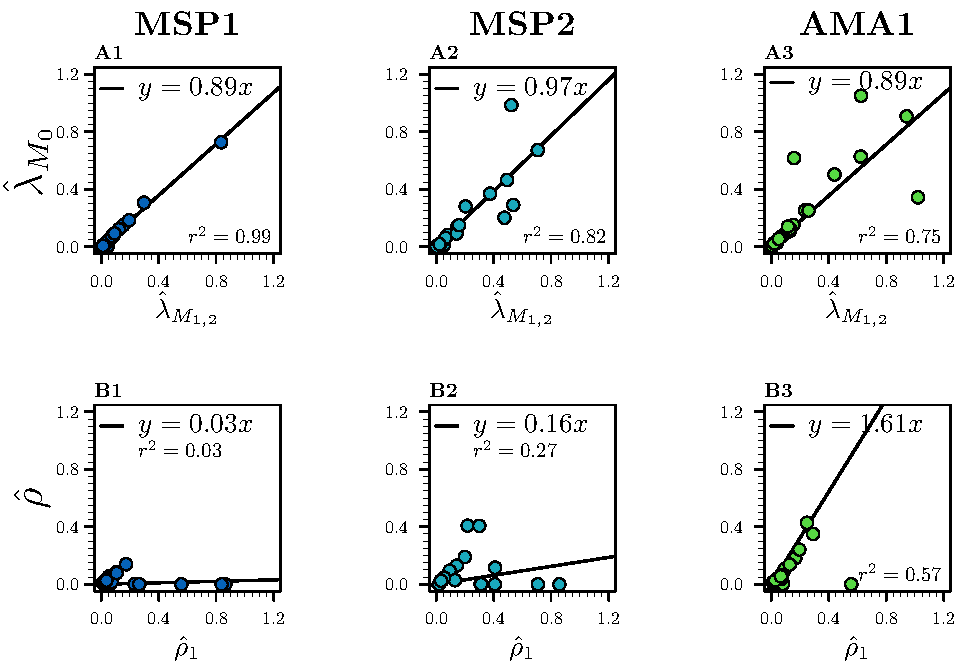
\includegraphics[width=\columnwidth]{images/M0vM12.pdf}
\end{adjustbox}
\caption[Correlation analyses between parameter estimates from M$_0$ and M$_ {1,2}$]{Comparison of parameter estimates from models M$_0$ and M$_{1,2}$. The first column, with figures \textbf{A1} and \textbf{B1}, represents analyses made for the MSP1 antigen data set, the second column, with figures \textbf{A2} and \textbf{B2}, represents analyses using the MSP2 antigen data, and third column, with figures \textbf{A3} and \textbf{B3}, represents analyses for the AMA1 antigen data set. Figures \textbf{A1}, \textbf{A2}, and \textbf{A3} in the first row, shows the 21 model M$_0$ SCR estimates, $ \widehat{\lambda}_{M_0}$, as function of the corresponding M$_{1,2}$ estimates. Figures \textbf{B1}, \textbf{B2}, and \textbf{B3} in the second row represent model M$_0$ SRR estimates, $ \widehat{\rho}$, as function of the M$_{1,2}$'s $ \widehat{\rho}_1$, calculated before the cutoff value $ \widehat{\uptau}$. For the second row, villages with $ \widehat{\rho}_1>10$ were excluded form the analysis. For each graph the line of tendency (in black) with respective formula and corresponding Pearson's correlation statistics, $r^2$, is shown.}
\label{fig:comparisons.M0.M12}
\end{figure}


%%%%% MSP1 %%%%%
\begin{sidewaystable}
\centering
\caption[Likelihood ratio test for comparing RCMs M$_0$ and M$_{1,2}$, MSP1 antigen data]{Comparison between models M$_0$ and M$_{1,2}$ using the likelihood ratio test. Data used from the immune responses to \textit{P. falciparum}-MSP1 antigen in samples from the 21 villages. Model M$_0$ assumes a constant SCR and SRR ($\lambda$ and $\rho$, respectively), while model M$_{1,2}$ assumes a constant SCR, $\lambda_1$ for ages $<\uptau$ and $\lambda_2=0$ otherwise. LogL refers to the log-likelihood function evaluated at the respective maximum likelihood estimates using profile likelihood method. P-value is associated with the log-likelihood ratio test comparing the nested model M$_0$ with M$_{1,2}$. Estimated 95\% confidence intervals including $>$10 suggest the model did not have sufficient information to accurately estimate the lower and upper limits. This event can be mostly seen at high altitude villages.}
\label{tab:M0.M12.msp1}
\begin{adjustbox}{width=\linewidth}
%%%%%%%%%%%%%%%%%%%%%%%%%%%
%%%%% MSP1 - M0 vs M12 %%%%
%%%%%%%%%%%%%%%%%%%%%%%%%%%
\begin{tabular}{llllllllclr} 
\toprule
\multicolumn{1}{c}{\multirow{2}{*}{Transect}} & \multicolumn{1}{c}{\multirow{2}{*}{Village}} & \multicolumn{3}{c}{Model M$_{0}$} & \multicolumn{1}{c}{} & \multicolumn{4}{c}{Model M$_{1,2}$} & \multicolumn{1}{c}{\multirow{2}{*}{p-value}}  \\ 
\cmidrule{3-5}\cmidrule{7-10}
\multicolumn{1}{c}{} & \multicolumn{1}{c}{} & \multicolumn{1}{c}{$\hat{\lambda}$ (95\% CI)} & \multicolumn{1}{c}{$\hat{\rho}$ (95\% CI)} & \multicolumn{1}{c}{logL} & \multicolumn{1}{c}{} & \multicolumn{1}{c}{$\hat{\lambda}$ (95\% CI)} & \multicolumn{1}{c}{$\hat{\rho}_1$ (95\% CI)} & \multicolumn{1}{c}{$\hat{\uptau}$} & \multicolumn{1}{c}{logL} & \multicolumn{1}{c}{} \\
\midrule
Rombo       & Mokala          & 0.014 (0.008, 0.030)   & 0.016 (0.000, 0.093)   & -45.68   & & 0.016 (0.009, $>$5)   & 0.031 (0.000, $>$10)   & 30 & -45.63 & 0.752\\
              & Machame Aleni & 0.047 (0.024, 0.140)   & 0.083 (0.020, 0.372)   & -56.54   & & 0.052 (0.027, $>$5)   & 0.104 (0.031, 0.460)   & 37 & -56.01 & 0.303\\
              & Ikuini        & 0.014 (0.010, 0.038)   & 0.000 (0.000, 0.102)   & -58.55   & & 0.020 (0.011, $>$5)   & 0.061 (0.000, $>$10)   & 22 & -58.16 & 0.377\\
              & Kileo         & 0.307 (0.205, 0.499)   & 0.055 (0.023, 0.125)   & -44.77   & & 0.298 (0.210, $>$5)   & 0.055 (0.026, 0.110)   & 40 & -45.61 & $\sim$1.000\\
\cmidrule{2-11}
N. Pare     & Kilomeni        & 0.005 (0.002, 0.038)   & 0.000 (0.000, 0.351)   & -18.93   & & 0.046 (0.004, $>$5)   & 0.864 (0.000, $>$10)   & 30 & -17.22 & 0.064\\
            & Lambo           & 0.015 (0.010, 0.041)   & 0.001 (0.000, 0.104)   & -37.86   & & 0.019 (0.010, $>$5)   & 0.232 (0.000, $>$10)   & 7  & -37.60 & 0.471\\
            & Ngulu           & 0.074 (0.046, 0.159)   & 0.000 (0.000, 0.058)   & -13.79   & & 0.084 (0.052, $>$5)   & $>$10 (0.000, $>$10)   & 1  & -13.31 & 0.327\\
            & Kambi ya Simba  & 0.067 (0.039, 0.122)   & 0.010 (0.000, 0.059)   & -27.45   & & 0.074 (0.043, $>$5)   & 0.019 (0.000, $>$10)   & 36 & -27.01 & 0.348\\
\cmidrule{2-11}
S. Pare     & Bwambo          & 0.005 (0.003, 0.017)   & 0.000 (0.000, 0.126)   & -36.14   & & 0.017 (0.004, $>$5)   & 0.265 (0.000, $>$10)   & 27 & -34.93 & 0.120\\
            & Mpinji          & 0.005 (0.002, 0.009)   & 0.000 (0.000, 0.055)   & -21.75   & & 0.009 (0.005, $>$5)   & $>$10 (0.134, $>$15)   & 8  & -19.23 & 0.025\\
            & Goha            & 0.032 (0.021, 0.054)   & 0.017 (0.000, 0.070)   & -58.55   & & 0.042 (0.025, $>$5)   & 0.073 (0.000, 0.196)   & 24 & -57.35 & 0.121\\
            & Kadando         & 0.152 (0.108, 0.230)   & 0.029 (0.011, 0.068)   & -57.05   & & 0.156 (0.115, $>$5)   & 0.032 (0.014, 0.069)   & 38 & -56.82 & 0.498\\
\cmidrule{2-11}
W. Usamb. 1 & Emmao           & 0.001 (0.000, 0.127)   & 0.000 (0.000, $>$10)   & -10.86   & & 0.006 (0.001, $>$5)   & 0.838 (0.000, $>$10)   & 26 &  -9.68 & 0.124\\
            & Handei          & 0.044 (0.021, 0.128)   & 0.139 (0.040, 0.520)   & -57.56   & & 0.049 (0.025, $>$5)   & 0.173 (0.062, 0.527)   & 37 & -56.42 & 0.131\\
            & Tewe            & 0.026 (0.020, 0.040)   & 0.000 (0.000, 0.032)   & -64.19   & & 0.030 (0.023, $>$5)   & $>$10 (0.000, $>$10)   & 2  & -62.63 & 0.077\\
            & Mn'galo         & 0.074 (0.056, 0.099)   & 0.009 (0.000, 0.026)   & -67.23   & & 0.075 (0.058, $>$5)   & 0.010 (0.000, $>$10)   & 40 & -67.08 & 0.584\\
\cmidrule{2-11}
W. Usamb. 2 & Kwadoe          & 0.007 (0.004, 0.011)   & 0.000 (0.000, 0.032)   & -37.52   & & 0.013 (0.007, $>$5)   & 0.558 (0.013, 2.794)   & 14 & -35.47 & 0.043\\
            & Funta           & 0.121 (0.088, 0.172)   & 0.018 (0.005, 0.045)   & -47.92   & & 0.123 (0.093, 0.169)  & 0.020 (0.007, 0.045)   & 40 & -47.46 & 0.337\\
            & Tamota          & 0.093 (0.063, 0.152)   & 0.041 (0.014, 0.100)   & -64.58   & & 0.092 (0.066, $>$5)   & 0.042 (0.017, 0.091)   & 40 & -65.06 & $\sim$1.000\\
            & Mgila           & 0.184 (0.131, 0.286)   & 0.026 (0.008, 0.070)   & -64.36   & & 0.194 (0.140, $>$5)   & 0.036 (0.013, 0.091)   & 33 & -64.45 & $\sim$1.000\\
\cmidrule{2-11}
W. Usamb. 3 & Mgome           & 0.727 (0.398, 4.520)   & 0.078 (0.023, 0.482)   & -34.25   & & 0.835 (0.457, $>$5)   & 0.107 (0.035, $>$10)   & 37 & -32.48 & 0.060\\
\bottomrule
\end{tabular}
\end{adjustbox}
\end{sidewaystable}

\newpage

%%%%% Figure %%%%%
\begin{figure}[H]
\center
\begin{adjustbox}{width=\linewidth,totalheight=\textheight-4\baselineskip}
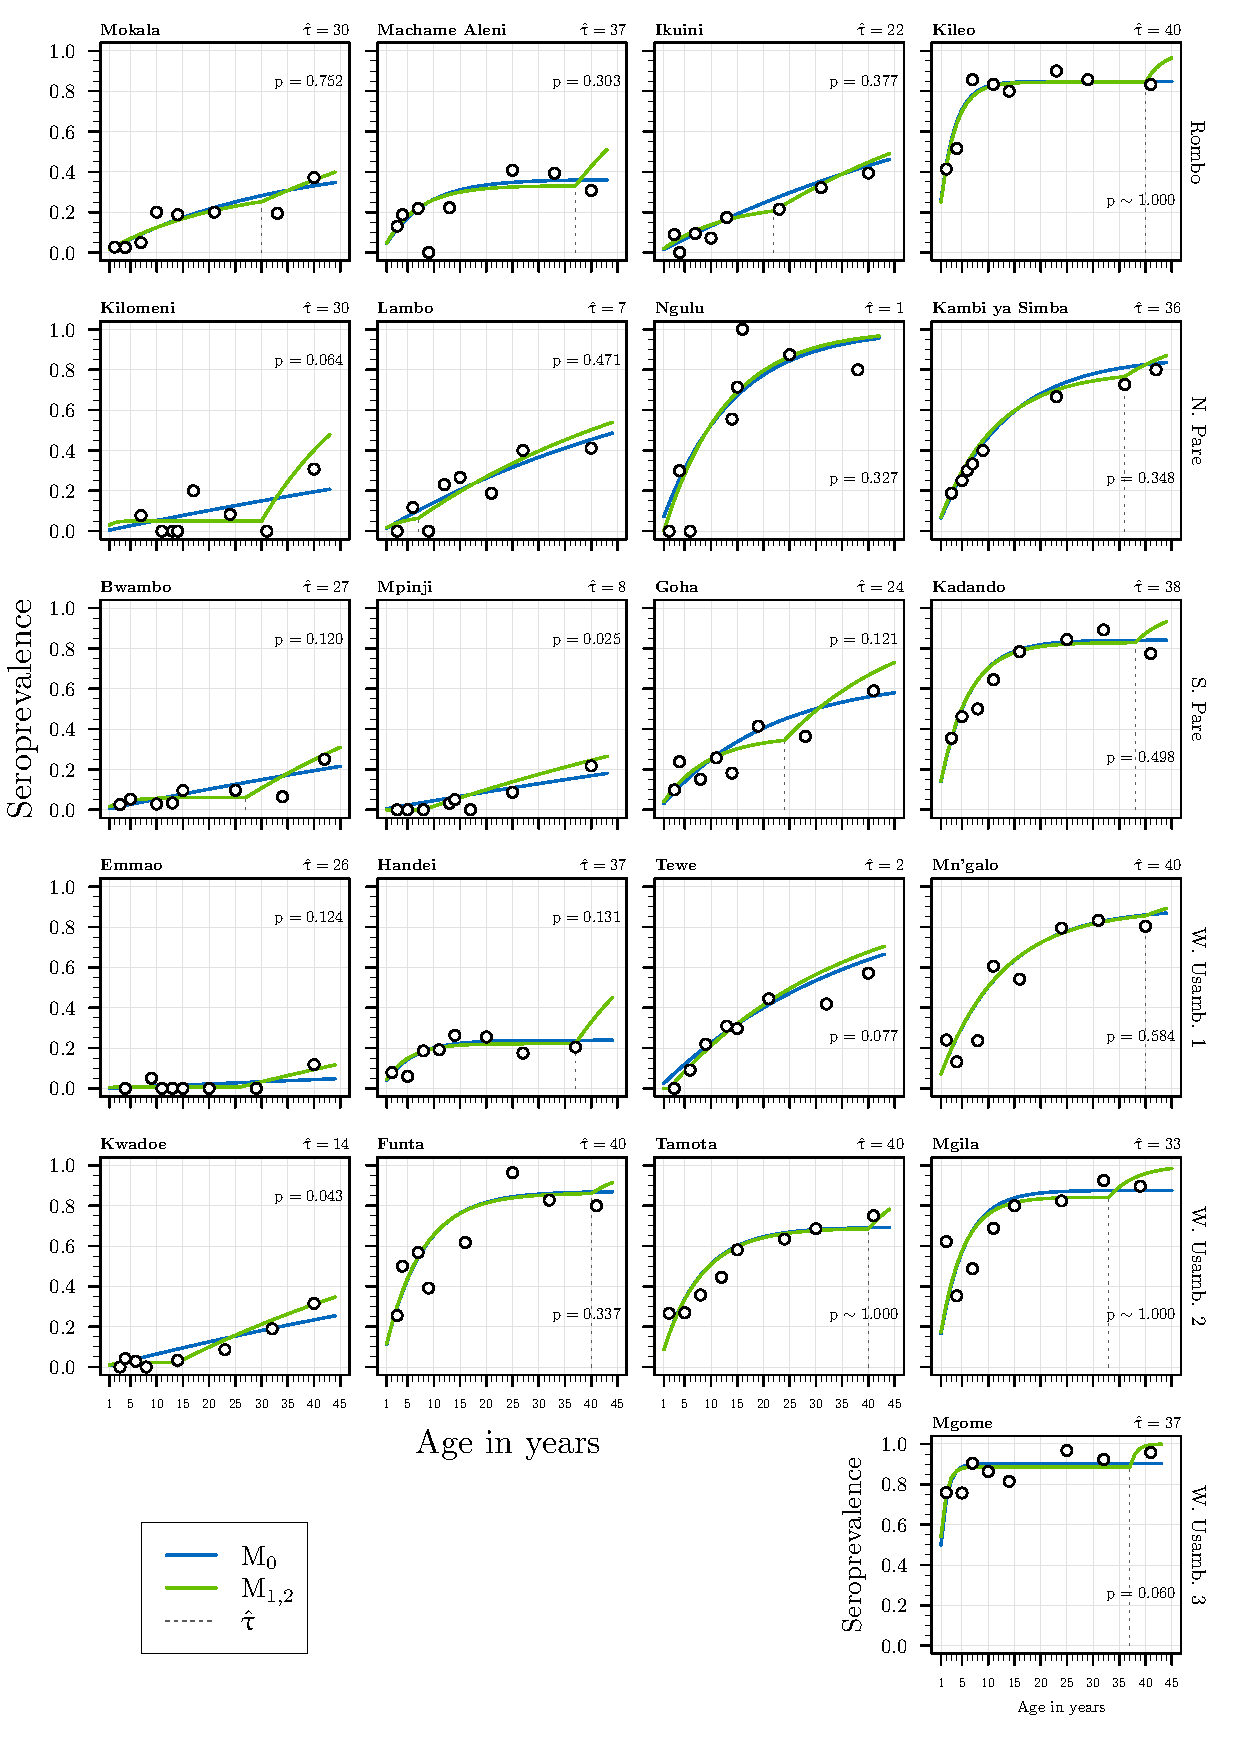
\includegraphics[width=\columnwidth]{images/Seroprevalence_M0vM12_msp1.pdf}
\end{adjustbox}
\caption[Estimated MSP1 seroprevalence for models M$_0$ and M$_{1,2}$]{Fits for the estimated MSP1 antigen seroprevalence for the 21 assessed villages, using models M$_0$ (blue lines) and M$_{1,2}$ (green lines), with the cutoff parameter of the latter signalled. Each row of graphs represents data from the transects (identified on the right hand side), where villages are ordered by decreasing altitude (and increasing malaria incidence). In the different plots, the dots represent the observed seroprevalence of distinct age groups by splitting the sampled age distribution into similar bins. P-values from the resulting likelihood ratio tests are identified.}
\label{fig:msp1.seroprevalence.M0.M12}
\end{figure}

\newpage


%%%%%%%%%%%
% M0 v M2 %
%%%%%%%%%%%
\subsection[Testing change in seroconversion rate]{Testing change in SCR: M$_{0}$ \textit{vs.} M$_{2}$}

% With the change in SRR statistically non significant,
With a possible change in SRR discarded for most villages, model M$_0$ was compared against M$_2$ to test if the SCR in each village was reasonably constant throughout the past years (Table \ref{tab:M0.M2.msp1} for MSP1, and from Appendices \ref{appendix:M0vM2}, Tables \ref{tab:M0.M12.msp2} and \ref{tab:M0.M12.ama1} for MSP2 and AMA1, respectively).
Model M$_2$ was developed assuming a change in SCR occurred some time before the sampling.
% Such cahange be originated from a successful campaign for prevention and control of the disease.
% The sudden change in SCR exposes individuals to a different intensity of malaria transmission.
% and adjust their immunological system accordingly.
Based on the frequency of antigens detected at different ages, model M$_2$ was able to estimate how long ago that change occurred, assuming $1\leq \widehat{\uptau}^*\leq40$.
% \textcolor{red}{, and how abrupt it was; isto aqui não faz sentido, a change pode ser positiva ou negativa}.

The estimated seroprevalence curves produced by this model suggested that a change in transmission might have occurred in various villages (Figure \ref{fig:seroprevalence.M0.M2} for the estimated seroprevalence from MSP1, and Figures \ref{fig:msp2.seroprevalence.M0.M2} and \ref{fig:ama1.seroprevalence.M0.M2} from Appendices \ref{appendix:M2.seroprev.msp2} and \ref{appendix:M2.seroprev.ama1}, respectively, for estimated seroprevalence from MSP2 and AMA1).
However, from the likelihood ratio tests, the apparently evident changes in SCR seen in model M$_2$ were in fact only statistically significant for a few villages.
% The different immunogenic antigens presented different villages where a significant change may have occurred.
Results from the MSP1 antigen identified a significant change in SCR in Kwadoe, Tamota, Mgila (all from transect West Usambara 2), and Mgome (West Usambara 3).
Estimates for Kwadoe ($ \widehat{\uptau}^*=30$) indicated the SCR reduction occurred approximately between 27 and 32 years before sampling (Figure \ref{fig:profile.kwadoe}).
The remaining three villages estimated the cutoff for change in SCR between one and two years ($ \widehat{\uptau}^*=1$).
For the MSP2 data set, villages Bwambo ($ \widehat{\uptau}^*=37$) and Mpinji ($ \widehat{\uptau}^*=1$) from the South Pare transect, and Funta ($ \widehat{\uptau}^*=6$) and Tamota ($ \widehat{\uptau}^*=1$), both from West Usambara 2, were identified.
In Bwambo, the SCR reduction took place between 35 and 39 years before the survey sampling.
Similar to the lower altitude villages identified using the previous antigen, the changes in Mpinji and, once again, in Tamota were estimated to approximately occur just one to two years before the data collection.
And in Tamota, a the gange in SCR occurred approximately six years before the study.
Likelihood ratio tests from the AMA1 antigen suggested that only individuals from the village Machame Aleni ($ \widehat{\uptau}^*=20$), from the transect Rombo, were exposed to a significant reduction in SCR during the last 40 years.
This change was estimated to happen approximately 20 years before sampling.



% As the more immunogenic, AMA1 is expected to be more easily detected at lower intensities of transmission, where other antigens might be significantly reduced.
% This sensitivity have resulted in less significant or noticeable changes in seroprevalence estimation.
% Non significant changes in SCR for AMA1 antigens have also been reported in \textit{P. vivax} analyses, under similar conditions \cite{cook2010using}.

% Despite the parametric restriction proposed for model M$_2$ ($\lambda_1\geq\lambda_2$), some villages where $\uptau^*$ was equal to one, estimated $\lambda_2$ with a higher value than $\lambda_1$.
% Although not intended, by occurring almost entirely on medium to low altitude villages, this event could grant some information about the sites.
% In those villages, children between one and two years old represented the interval where model M$_2$ identified the greatest change in SCR across all ages.
% % This event ($\uptau^*=1$) causes M$_2$ to estimate seroprevalence using only the upper bracket from equation (\ref{eq:rcm.reduction.scr}).
% The seroprevalence curves generated under this assumption ($\uptau^*=1$) did not present the characteristic biphasic behaviour from M$_2$ (Figure \ref{fig:seroprevalence.M0.M12}).
% An example was the village Tamota.
% Despite a statistically significant change in SCR for two antigens, with an estimated cutoff equal to one, its maximum likelihood estimators for $\lambda_2$ were higher than $\lambda_1$ in both occasions.
% This could also be malfunction from the package, due to the small amount of information available to perform more precise estimations at each year.

%%%%% MSP1 %%%%%
\begin{sidewaystable}
\centering
\caption[Likelihood ratio test for comparing RCMs M$_0$ and M$_{2}$, MSP1 antigen data]{Comparative analysis of the results from models  M$_{0}$ and M$_{2}$, referring all 21 villages, considering MSP1 individual status as the outcomes. Model M$_{0}$ assumes constant SCR ($\lambda$) and SRR ($\rho$) for all ages. Model M$_{2}$ also assumes constant SRR, and a change in SCR after the cutoff parameter, $\uptau^*$. logL refers to the log-likelihood function evaluated at the respective maximum likelihood estimates using the profile likelihood method. p-value is associated with the log-likelihood ratio test comparing both models.}
\label{tab:M0.M2.msp1}
\begin{adjustbox}{width=\linewidth}
%%%%%%%%%%%%%%%%%%%%%%%%%%
%%%%% MSP1 - M0 vs M2 %%%%
%%%%%%%%%%%%%%%%%%%%%%%%%%
\begin{tabular}{lllllllllclr}
\toprule
\multicolumn{1}{c}{\multirow{2}{*}{Transect}} & \multicolumn{1}{c}{\multirow{2}{*}{Village}} & \multicolumn{3}{c}{Model M$_0$} & \multicolumn{1}{c}{} & \multicolumn{5}{c}{Model M$_2$} & \multicolumn{1}{c}{\multirow{2}{*}{p-value}}  \\ 
\cmidrule{3-5}\cmidrule{7-11}
\multicolumn{1}{c}{} & \multicolumn{1}{c}{} & \multicolumn{1}{c}{$\hat{\lambda}$ (95\% CI)} & \multicolumn{1}{c}{$\hat{\rho}$ (95\% CI)} & \multicolumn{1}{c}{logL} & \multicolumn{1}{c}{} & \multicolumn{1}{c}{$\hat{\lambda}_1$ (95\% CI)} & \multicolumn{1}{c}{$\hat{\lambda}_2$ (95\% CI)} & \multicolumn{1}{c}{$\hat{\rho}$ (95\% CI)} & \multicolumn{1}{c}{$\hat{\uptau}^*$} & \multicolumn{1}{c}{logL} & \multicolumn{1}{c}{} \\ 
\midrule
Rombo       & Mokala         & 0.014 (0.008, 0.030)   & 0.016 (0.000, 0.093)   & -45.68   & &   100.664 (0.006, $>$10) & 0.012 (0.004, 0.031)   & 0.190 (0.000, 0.243)   & 8   & -44.43   & 0.287\\
            & Machame Aleni  & 0.047 (0.024, 0.140)   & 0.083 (0.020, 0.372)   & -56.54   & &   54.484 (0.000, $>$10)  & 0.045 (0.026, 0.085)   & 0.107 (0.031, 0.203)   & 14  & -55.23   & 0.270\\
            & Ikuini         & 0.014 (0.010, 0.038)   & 0.000 (0.000, 0.102)   & -58.55   & &   0.011 (0.006, 0.025)   & 0.051 (0.012, 0.116)   & 0.000 (0.000, 0.053)   & 1   & -56.88   & 0.188\\
            & Kileo          & 0.307 (0.205, 0.499)   & 0.055 (0.023, 0.125)   & -44.77   & &   236.197 (0.122, $>$10) & 0.287 (0.184, 0.449)   & 0.077 (0.031, 0.127)   & 4   & -43.83   & 0.391\\
\cmidrule{2-12}
N. Pare     & Kilomeni       & 0.005 (0.002, 0.038)   & 0.000 (0.000, 0.351)   & -18.93   & &   0.027 (0.000, $>$10)   & 0.004 (0.001, 0.013)   & 0.003 (0.000, 0.103)   & 27  & -17.84   & 0.336\\
            & Lambo          & 0.015 (0.010, 0.041)   & 0.001 (0.000, 0.104)   & -37.86   & &   78.671 (0.000, $>$10)  & 0.010 (0.002, 0.035)   & 0.125 (0.000, 0.180)   & 10  & -36.47   & 0.249\\
            & Ngulu          & 0.074 (0.046, 0.159)   & 0.000 (0.000, 0.058)   & -13.79   & &   58.997 (0.071, $>$10)  & 0.038 (0.009, 0.105)   & 0.018 (0.000, 0.046)   & 13  & -11.88   & 0.148\\
            & Kambi ya Simba & 0.067 (0.039, 0.122)   & 0.010 (0.000, 0.059)   & -27.45   & &   44.179 (0.000, $>$10)  & 0.068 (0.040, 0.112)   & 0.023 (0.000, 0.055)   & 17  & -27.02   & 0.651\\
\cmidrule{2-12}
S. Pare     & Bwambo         & 0.005 (0.003, 0.017)   & 0.000 (0.000, 0.126)   & -36.14   & &   20.786 (0.000, $>$10)  & 0.006 (0.003, 0.011)   & 0.039 (0.000, 0.070)   & 35  & -33.49   & 0.071\\
            & Mpinji         & 0.005 (0.002, 0.009)   & 0.000 (0.000, 0.055)   & -21.75   & &   1.962 (0.008, $>$10)   & 0.003 (0.001, 0.008)   & 0.058 (0.000, 0.092)   & 24  & -18.88   & 0.057\\
            & Goha           & 0.032 (0.021, 0.054)   & 0.017 (0.000, 0.070)   & -58.55   & &   0.019 (0.012, 0.036)   & 0.061 (0.029, 0.102)   & 0.000 (0.000, 0.034)   & 2   & -56.59   & 0.141\\
            & Kadando        & 0.152 (0.108, 0.230)   & 0.029 (0.011, 0.068)   & -57.05   & &   0.093 (0.046, 0.161)   & 0.343 (0.164, 0.575)   & 0.018 (0.000, 0.046)   & 1   & -54.54   & 0.081\\
\cmidrule{2-12}
W. Usamb. 1 & Emmao          & 0.001 (0.000, 0.127)   & 0.000 (0.000, $>$10)   & -10.86   & &   24.373 (0.000, $>$10)  & 0.001 (0.000, 0.005)   & 0.081 (0.000, 0.219)   & 30  & -9.35    & 0.221\\
            & Handei         & 0.044 (0.021, 0.128)   & 0.139 (0.040, 0.520)   & -57.56   & &   117.997 (0.000, $>$10) & 0.047 (0.022, 0.100)   & 0.282 (0.000, 0.434)   & 7   & -56.68   & 0.415\\
            & Tewe           & 0.026 (0.020, 0.040)   & 0.000 (0.000, 0.032)   & -64.19   & &   0.048 (0.026, 0.089)   & 0.000 (0.000, 0.022)   & 0.022 (0.000, 0.065)   & 3   & -61.72   & 0.085\\
            & Mn'galo        & 0.074 (0.056, 0.099)   & 0.009 (0.000, 0.026)   & -67.23   & &   50.536 (0.167, $>$10)  & 0.071 (0.054, 0.092)   & 0.022 (0.014, 0.034)   & 15  & -64.46   & 0.063\\
\cmidrule{2-12}
W. Usamb. 2 & Kwadoe         & 0.007 (0.004, 0.011)   & 0.000 (0.000, 0.032)   & -37.52   & &   2.652 (0.299, $>$10)   & 0.004 (0.002, 0.008)   & 0.038 (0.026, 0.056)   & 30  & -31.49   & 0.002\\
            & Funta          & 0.121 (0.088, 0.172)   & 0.018 (0.005, 0.045)   & -47.92   & &   59.081 (0.000, $>$10)  & 0.116 (0.087, 0.157)   & 0.022 (0.011, 0.042)   & 13  & -46.53   & 0.249\\
            & Tamota         & 0.093 (0.063, 0.152)   & 0.041 (0.014, 0.100)   & -64.58   & &   0.046 (0.023, 0.084)   & 0.243 (0.128, 0.389)   & 0.016 (0.000, 0.051)   & 1   & -60.30   & 0.014\\
            & Mgila          & 0.184 (0.131, 0.286)   & 0.026 (0.008, 0.070)   & -64.36   & &   0.062 (0.038, 0.110)   & 0.579 (0.378, 0.807)   & 0.002 (0.000, 0.023)   & 1   & -53.04   & $<$0.001\\
\cmidrule{2-12}
W. Usamb. 3 & Mgome          & 0.727 (0.398, 4.520)   & 0.078 (0.023, 0.482)   & -34.25   & &   0.088 (0.023, 0.432)   & 1.310 (0.748, 1.847)   & 0.010 (0.000, 0.088)   & 1   & -30.86   & 0.034\\
\bottomrule
\end{tabular}
\end{adjustbox}
\end{sidewaystable}

\newpage

%%%%% Figure %%%%%
\begin{figure}[H]
\center
\begin{adjustbox}{width=\linewidth,totalheight=\textheight-5\baselineskip}
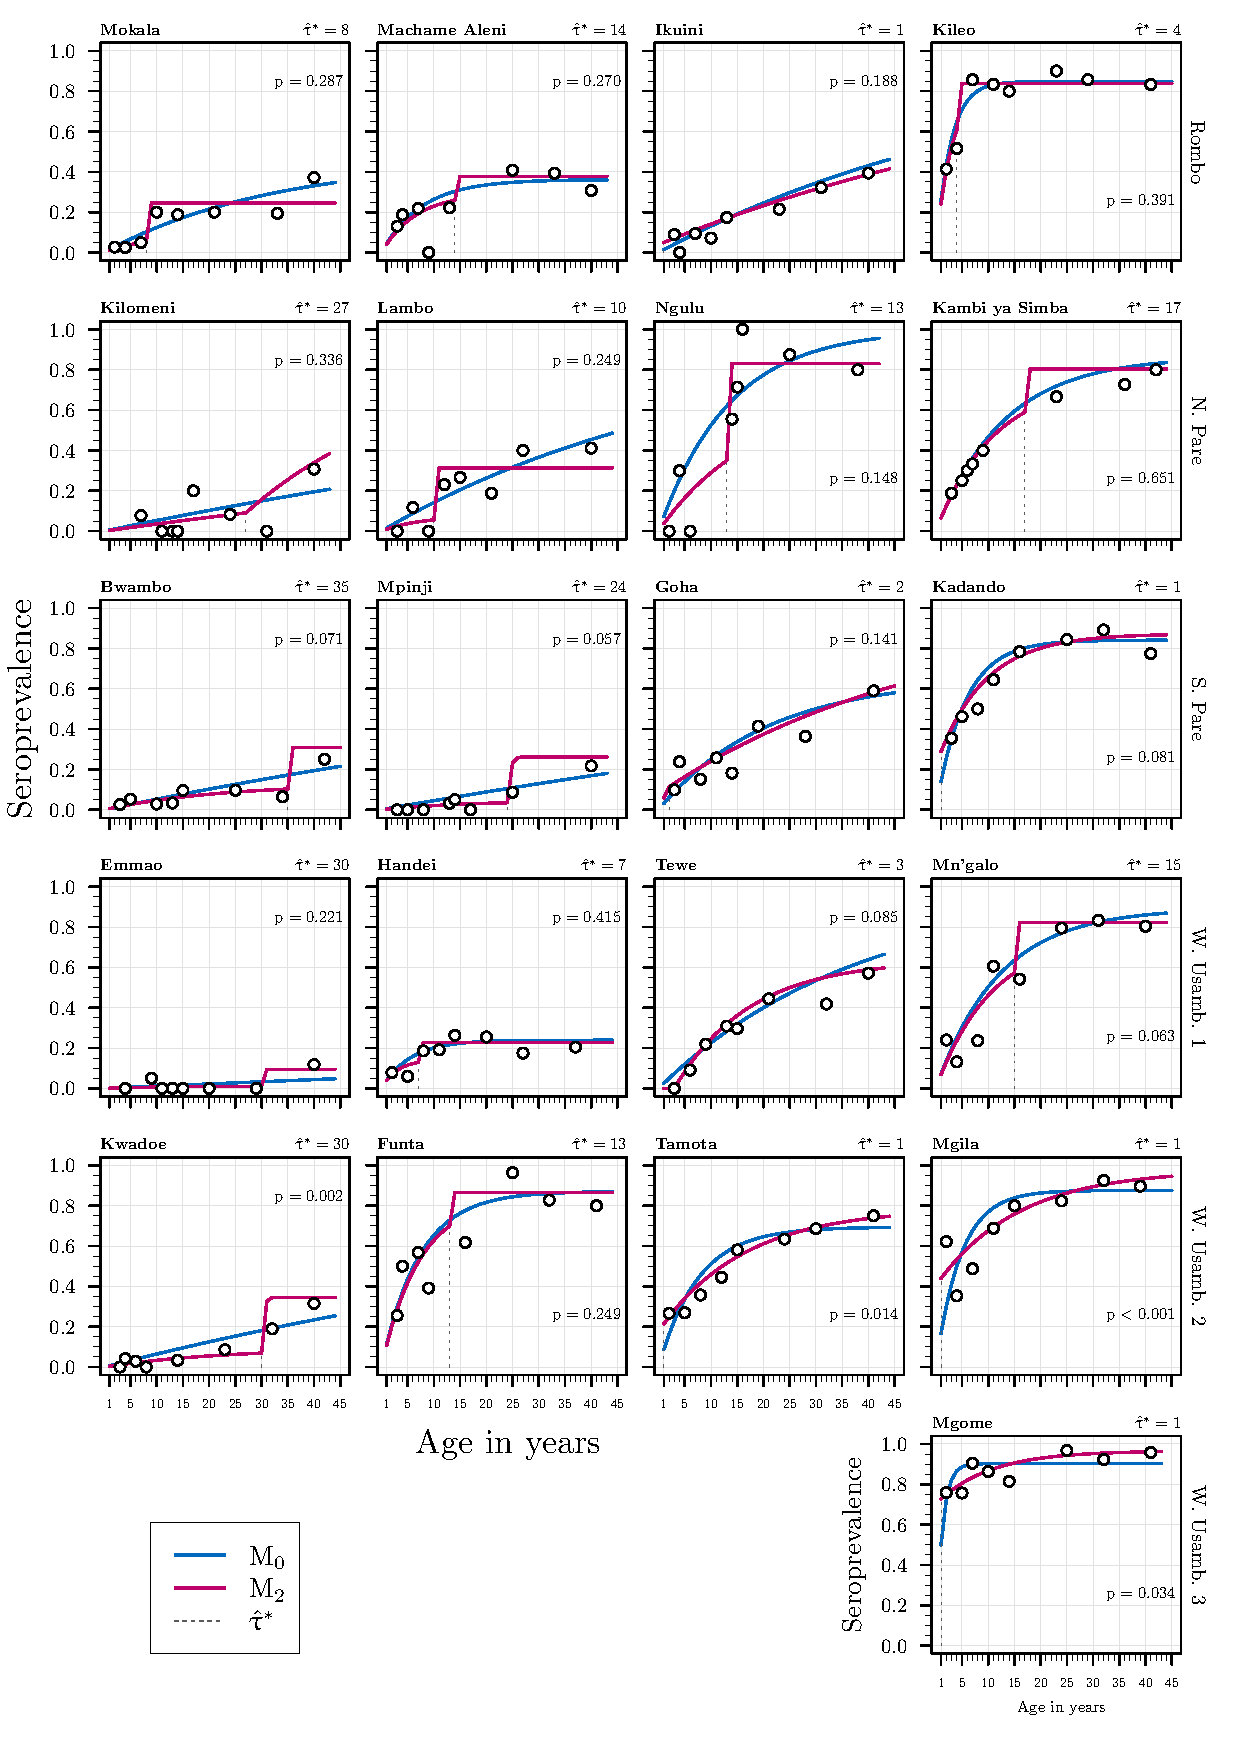
\includegraphics[width=\columnwidth]{images/Seroprevalence_M0vM2_msp1.pdf}
\end{adjustbox}
\caption[Estimated MSP1 seroprevalence for models M$_0$ and M$_2$]{Fits for the estimated MSP1 antigen seroprevalence for the 21 assessed villages, using models M$_0$ (blue lines) and M$_2$ (light red lines), with the cutoff parameter of the latter signalled, identifying the change in SCR happening in years before sampling. Each row of graphs represents data from the transects (identified on the right hand side), where villages are ordered by decreasing altitude (and increasing malaria incidence). In the different plots, the dots represent the observed seroprevalence of distinct age groups by splitting the sampled age distribution into similar bins. P-values from the resulting likelihood ratio tests are identified.}
\label{fig:seroprevalence.M0.M2}
\end{figure}


\begin{figure}[ht!]
\center
\begin{adjustbox}{width=\linewidth}
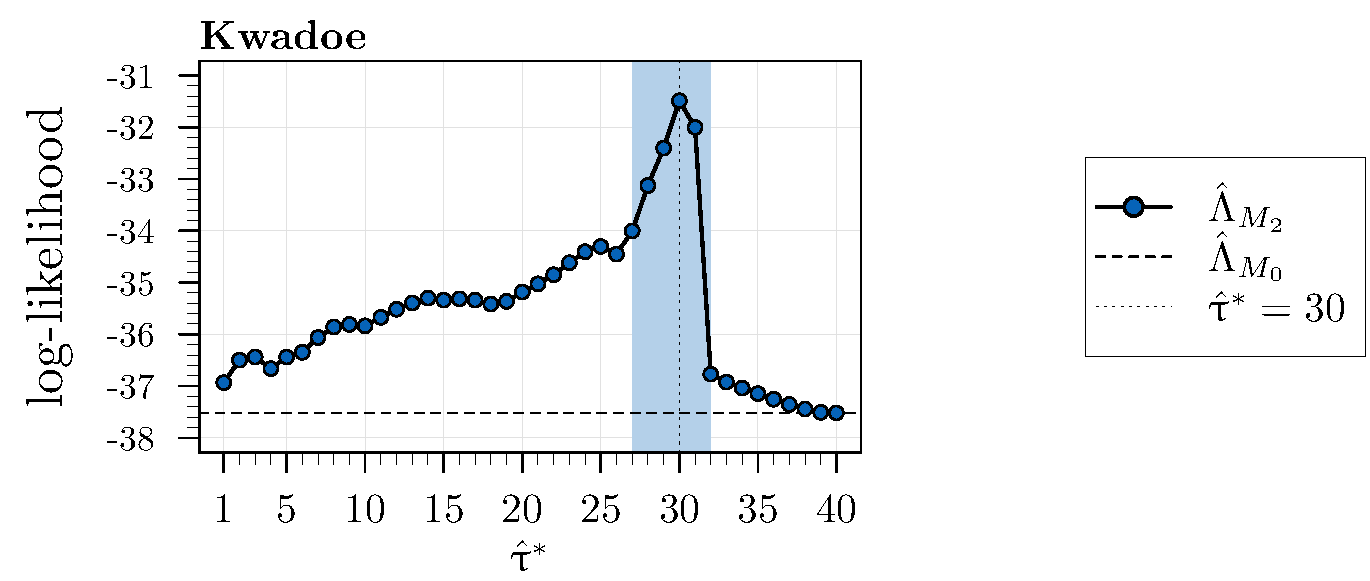
\includegraphics[width=\columnwidth]{images/profile_kwadoe.pdf}
\end{adjustbox}
\caption[Profile likelihood methodology for estimation of parameters from village Kwadoe, MSP1 antigen data]{Example of the profile likelihood methodology implemented to estimate parameter values from village Kwadoe in model M$_2$. Parameters that maximised the log-likelihood were estimated by gradually increasing one unit in the cutoff parameter $\uptau^*$ and estimate the remaining parameters $\lambda_1$, $\lambda_2$, and $\rho$ at each level, via maximum likelihood. Estimate $ \widehat{\uptau}^*=30$ (thin dashed line) returns the maximum value of log-likelihood and all the associated parameters. The Horizontal dashed line represents the maximum log-likelihood estimated using model M$_0$, under the same data set.}
\label{fig:profile.kwadoe}
\end{figure}

%%%%%%%%%%%%%
%% M12 v M2 %
%%%%%%%%%%%%%
%\subsubsection{M$_{2}$ \textit{vs} M$_{1,2}$}
%Tenho esta comparação. Are they nested? Is it worth it?
%Testing for evident changes in SRR and SCR by comparing models M$_{1,2}$ and M$_{2}$ against M$_{0}$ has shown that for most situations, the simpler model is the more parsimonious one.
%%%%%% MSP1 %%%%%
%\begin{sidewaystable}
%\centering
%\caption[Comparison of RCM models M$_{1,2}$ and M$_{2}$ applied to the MSP1 data set]{.}
%\label{tab:M12.M2.msp1}
%\begin{adjustbox}{width=\linewidth}
%\input{tables/table_M12vM2_msp1.tex}
%\end{adjustbox}
%\end{sidewaystable}
%
%%%%%% MSP2 %%%%%
%\begin{sidewaystable}
%\centering
%\caption[Comparison of RCM models M$_{1,2}$ and M$_{2}$ applied to the MSP2 data set]{Statistical analysis of the MSP2 antigen data set referring to the 21 Tanzanian villages.}
%\label{tab:M12.M2.msp2}
%\begin{adjustbox}{width=\linewidth}
%\input{tables/table_M12vM2_msp2.tex}
%\end{adjustbox}
%\end{sidewaystable}
%
%%%%%% AMA1 %%%%%
%\begin{sidewaystable}
%\centering
%\caption[Comparison of RCM models M$_{1,2}$ and M$_{2}$ applied to the AMA1 data set]{Statistical analysis of the AMA1 antigen data set referring to the 21 Tanzanian villages.}
%\label{tab:M12.M2.ama1}
%\begin{adjustbox}{width=\linewidth}
%\input{tables/table_M12vM2_ama1.tex}
%\end{adjustbox}
%\end{sidewaystable}

\section{Antibody seroprevalence as indicator of malaria transmission intensity}
% \textcolor{red}{E agora o que é que acontece à transmissão actual em cada uma das vilas? Como varia? What about interpretations about SCR for all villages? Pelo menos um parágrafo a explicar a transmissão! Meter a figura que enviei, analisar! Análise final: qual é a corelação entre prevalência de infecção e seroprevalence!!
% Devia mostrar prof likelihood para as vilas em que há uma redução significativa.}
% (Table \ref{tab:EIR.to.SCR} from Appendices)
% When assessing how malaria transmission rate behaves across the studied villages, the serology-based models characterise the populations' current state of transmission intensity by focusing on the presence/absence of specific malarial antigens.
% The RCMs went even further, describing how transmission intensity evolved across the sequence of ages, translating the estimated rates into age-specific seroprevalence values for each site.

With the more parsimonious serology-based model for each one of the studied villages identified, inferences about possible patterns in transmission intensity and how the seroprevalence evolved over time were performed.
Irrespective of the malarial antigen analysed, most villages were best described considering SCR and SRR as constant transition rates across all ages (model M$_0$).
An overall analysis on the model estimates implied a noticeable influence of altitude on the SCR, proxy for transmission intensity (Figure \ref{fig:M0.SCR.altitude}).
As seen when describing the age-dependent model M$_{1,2}$, SCR estimates suggested an inverse relation with altitude.
Similarly, the different $ \widehat{\lambda}$ estimates from M$_0$ presented moderate correlation with altitude ($r^2_{MSP1}=0.46$, $r^2_{MSP2}=0.42$, and $r^2_{AMA1}=0.48$).
The analysis between the estimates produced with different antigens corroborated a conclusion made in Chapter \ref{ch:4.0}, indicating AMA1 as the most immunogenic antigen of the three.
The SCR estimated when using the serological data for this antigen were consistently higher across all villages, when compared to the remaining antigens.
Meaning that even at high altitudes (lower transmission intensities), some levels of AMA1 antigens could be more easily detected in the individual's blood stream.
The results suggested MSP1 to be the less immunogenic, confirming the results observed during the exploratory analysis (Table \ref{tab:prevalence.seroprevalence} from Chapter \ref{ch:2.0}).

\begin{figure}[ht!]
\center
\begin{adjustbox}{width=\linewidth}
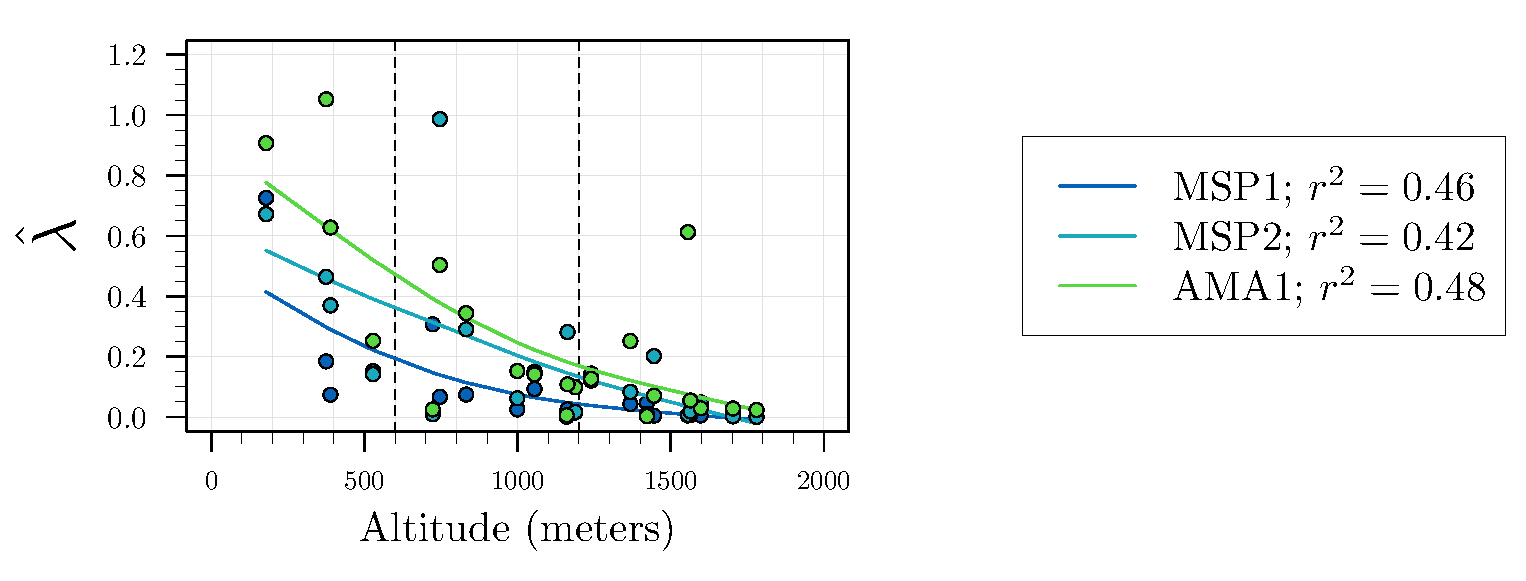
\includegraphics[width=\columnwidth]{images/M0_vs_altitude.pdf}
\end{adjustbox}
\caption[Dependency between altitude and SCR estimates]{Estimated SCR for each village using the RCM M$_0$. Each coloured point represents the transmission intensity estimated for each antigen data (MSP1, MSP2, and AMA1), as function of the respective village's altitude. The coloured lines are but an emphatic description of the transmission's trend. Vertical dashed lines represent the defined altitude limits, distinguishing between high ($>$1200m), medium (600m$-$1200m) and low ($<$600m) altitude villages.}
\label{fig:M0.SCR.altitude}
\end{figure}

Focusing on different transects encompassing clusters of altitude-defined villages, as well as some population genetic traits, transects from the Tanga region (West Usambara 1, 2, and 3) suggested higher estimated levels of transmission intensity.
More often villages from this region experienced a significant change in SCR some time before the sampling collection.
West Usambara 2 and West Usambara 3 (village Mgome), had their current estimates for SCR ($ \widehat{\lambda}$ or $ \widehat{\lambda}_2$, depending on the selected model) generally above $0.100$ in all data sets.
Transects from the Kilimanjaro region (transects Rombo, North, and South Pare) suggested lower estimates for transmission intensity.
Despite having similar structures in altitude, when compared to the villages from Tanga, the Kilimanjaro transects were located more inland, where a lesser humid climate is expected and could have presented an influence on the \textit{Anopheles} mosquitoes capacity.
The estimated values from Rombo relatively to the MSP1 data could suggest some affinity from individuals of the Wachaga ethnic group to produce the specific antibodies for the antigen.
The transmission intensities estimated in villages from this transect were notoriously higher, presenting similar levels to villages with higher measures of prevalence of infection.
However, the there was no strong discernible differences other than altitude and its effects on climate, that could indicate the reason for the different transmission intensities estimated.

%%%%%%%%%%%
% SUMMARY %
%%%%%%%%%%%
\section{Summary}

Comparing different nested RCMs to test biological and epidemiological hypotheses came to show that although seemingly close to a more realistic scenario, the effects of acquired immunity (model M$_{1,2}$), or past impacts from possible control measures (model M$_2$), did not present an impactful statistically significance, when applied to the data.
Model M$_0$ significantly described most of the studied villages.
Some exceptions were the villages Tamota and Mgila, best described by the RCM M$_2$, estimating that a recent change in SCR had occurred in the past years.
Model M$_{1,2}$ was also significant for some sites, describing villages located at intermediate and higher altitudes, such as Mpinji and Goha from the South Pare transect.

Correlation studies between M$_{1,2}$ and the more parsimonious M$_0$ suggested that neglecting to consider the age-dependent immunological uplift creates major underestimations in the SRR estimates, when considering the antigens MSP1 and MSP2.
% % Despite some villages evidencing a significant change in SCR, the overall best, model M$_0$, assumed both transition rates to be constant across all ages.
% The epidemiological proposal for past impacts able to effectively produce changes in malaria transmission was also dismissed for most villages.
% % Results based on this inference, modelled by M$_2$, were statistically non significant for the AMA1 data, with few villages from the MSP1$_{1,2}$ and MSP2 data sets deemed viable, when compared against M$_0$.
The simpler model M$_0$, with generally higher log-likelihoods than the remaining, more complex RCMs, is then considered the best model for the analysed data.
This conclusion implies that a more generalist model will prevail over other, more specialised proposals, when the population sample sizes under analysis do not provide sufficient data that would allow better estimations of parameters from the different models.
Results obtained by model M$_0$ demonstrated the dependency between the annual rate of seroconversion and altitude, with estimates for the AMA1 antigen being consistently higher than the others.
% \textcolor{red}{ tau^*==1 pode ser efeito dos maternal antibodies olhando figura 5.2. parece que o cutoff de idade de 1 ano poderá não ser o melhor cutoff Poderia ver a prevalência de infecção nos indivíduos com 1 ano de idade}.
% \textcolor{red}{TENHO DE POR CHAPÉU EM TODOS OS PARÂMETROS!!!!}
% Being the statistically more parsimonious, model M$_0$ presented underestimated parameter values when compared to M$_{1,2}$.
% It is worth mention the estimation of SRR has been shown difficult to estimate when using cross-sectional surveys.
% The difficulty can create some uncertainties when estimating the change point parameter $\uptau$, in the profile likelihood method.
% Are examples the model results for the MSP1 seroprevalence outcome (Table \ref{tab:M12.M11.msp1}), where both models estimate $\rho_1$ equal to zero at different cutoff values, for the villages Kilomeni, Ngulu, Mpinji, Tewe, and Kwadoe.
% As the more immunogenic, AMA1 is expected to be more easily detected at lower intensities of transmission, where other antigens might be significantly reduced.
% This sensitivity have resulted in less significant or noticeable changes in seroprevalence estimation.
% Non significant changes in SCR for AMA1 antigens have also been reported in \textit{P. vivax} analyses, under similar conditions \cite{cook2010using}.

% Despite the parametric restriction proposed for model M$_2$ ($\lambda_1\geq\lambda_2$), some villages where $\uptau^*$ was equal to one, estimated $\lambda_2$ with a higher value than $\lambda_1$.
% Although not intended, by occurring almost entirely on medium to low altitude villages, this event could grant some information about the sites.
% In those villages, children between one and two years old represented the interval where model M$_2$ identified the greatest change in SCR across all ages.
% % This event ($\uptau^*=1$) causes M$_2$ to estimate seroprevalence using only the upper bracket from equation (\ref{eq:rcm.reduction.scr}).
% The seroprevalence curves generated under this assumption ($\uptau^*=1$) did not present the characteristic biphasic behaviour from M$_2$ (Figure \ref{fig:seroprevalence.M0.M12}).
% An example was the village Tamota.
% Despite a statistically significant change in SCR for two antigens, with an estimated cutoff equal to one, its maximum likelihood estimators for $\lambda_2$ were higher than $\lambda_1$ in both occasions.
% This could also be malfunction from the package, due to the small amount of information available to perform more precise estimations at each year.
